% !TeX spellcheck = ru_RU
% !TEX root = vkr.tex

\section{Тестирование транслятора}

\begin{figure}[h]
    \begin{center}
        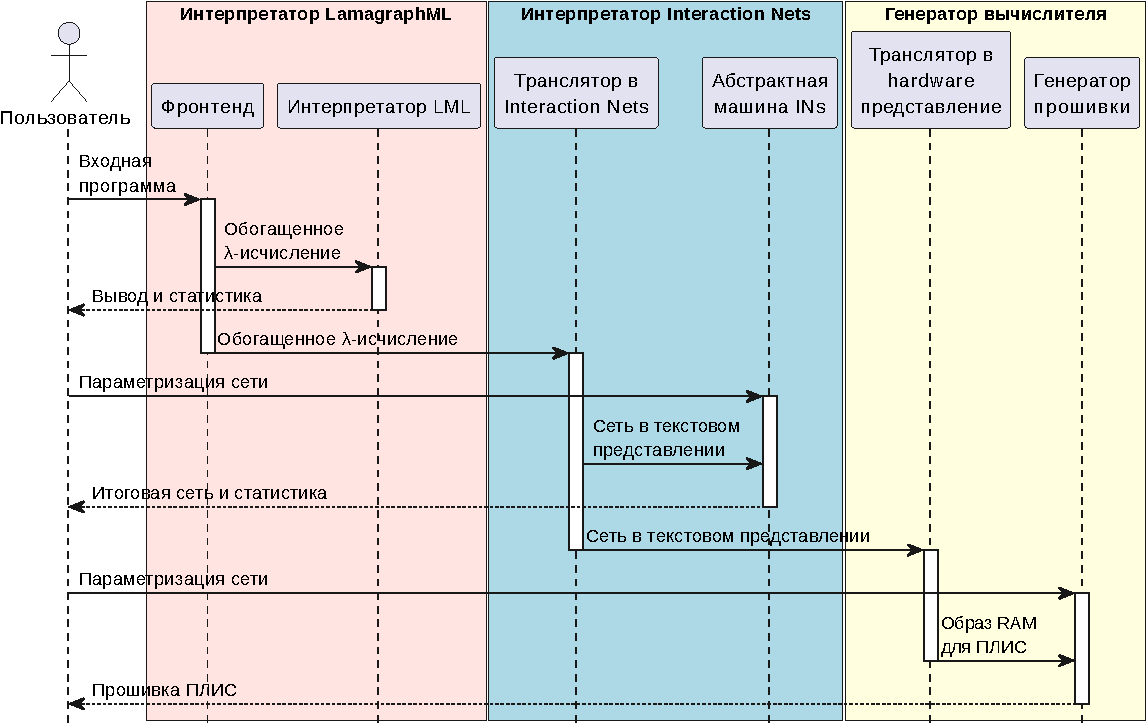
\includegraphics[width=0.9\linewidth]{using.pdf}
    \end{center}
    \caption{Диаграмма взаимодействия пользователя с программно-аппаратным стеком Lamagraph.}
    \label{fig:using}
\end{figure}

На данном этапе развития проекта проведение сравнительных экспериментов невозможно, тем не менее пользователь уже может взаимодействовать с инструментом.

Так, передав на вход программу на \LamagraphML{} пользователь может получить вывод интерпретатора, а также вывод абстрактной машины и соответствующую статистику, что проиллюстрировано на рисунке~\ref{fig:using}.

\subsection*{Анализ текущих возможностей}

Анализ проводился с учётом реализованной схемы трансляции чистого $\lambda$-исчисления в \INs{} со стратегией Call-by-Value.
Для вычисления использовались два набора правил: для последовательного вычисление аргументов применения и для параллельного.
Оба набора описаны в~\cite{sinotCallbyNameCallbyValueTokenPassing2005} и отличаются лишь правилом для взаимодействия агентов $\Downarrow$ и $a$.

\paragraph{Допустимые термы.}
Для проведения анализа было написано 10 программ.
Первоначально планировалось писать программы только на высокоуровневом \LamagraphML{}, однако в процессе выяснилось, что не все термы, используемые в бестиповом $\lambda$-исчислении могут быть протипизированы в системе типов Хиндли-Милнера без использования алгебраических типов данных (например, терм \texttt{pred}\footnote{Подробность можно прочитать в заметке Олега Киселева: \url{https://okmij.org/ftp/Computation/lambda-calc.html\#predecessor} (дата обращения: \DTMdate{2025-05-22})}).
Поэтому часть программ была вручную написана на бестиповом Core.
Кроме того, для корректного завершения программ в стратегии Call-by-Value условные конструкции необходимо было сделать \enquote{отложенными}, введя дополнительную $\lambda$-абстракцию\footnote{Более подробная мотивация такого подхода описана по ссылке: \url{https://cs.stackexchange.com/a/121350} (дата обращения: \DTMdate{2025-05-22})}.

Данная проблема~--- одна из самых важных для проекта на данный момент, поскольку Core и \INs{} планировалось использовать, как промежуточные представления, предоставляя пользователю только \LamagraphML{} и соответствующие возможности высокоуровневого языка.

Один из вариантов решения данной проблемы~--- введение числовых литералов, примитивных арифметических операцией и сопоставления с образцом.
Такое решение потребует расширения набора агентов и правил редукции, с учётом того, что арифметические операции строгие (eager) в своих аргументах.
Кроме того, необходимо изучить, каким образом возможна реализации такого расширения в компоненте Hardware.

\paragraph{Корректность результата.}
\begin{listing}
    \inputminted[fontsize=\footnotesize, breaklines]{ocaml}{figures/iterFactZero.lml}
    \caption{\texttt{IterFact(0)}, реализованный на \LamagraphML{}}
    \label{lst:iterFactZero}
\end{listing}
При анализе получаемых сетей была выявлена ещё одна проблема: Call-by-Value стратегия по определению не редуцирует под $\lambda$-абстракцией из-за чего получаемые сети довольно сложно анализировать на корректность ответа.

Так, например, в нотации из~\cite{fernandezCalculusInteractionNets1999}, результат вычисления итеративного факториала от 0 (см. листинг~\ref{lst:iterFactZero}) выглядит, как
\[\big\langle \Uparrow(\lambda(f, \lambda(x, a(f, x)))) \mid \big\rangle,\]
а для факториала от 1 уже так:
\begin{multline*}
    \big\langle \Uparrow(\lambda(f, \lambda(x, a(a(\lambda(c(u, v), \lambda(w, a(u, a(a(\lambda(\varepsilon, \lambda(z, z)), v), w)))), \\
    a(\lambda(t, \lambda(r, a(t, r))), f)), x)))) \mid \big\rangle.
\end{multline*}

В качестве решения проблемы можно, как уже упоминалось выше, добавить поддержку числовых литералов.
Также можно попробовать транслировать сеть обратно в $\lambda$-терм и осуществить оставшиеся редукции руками или с помощью интерпретатора, реализующего порядок вычислений, редуцирующий внутри $\lambda$-абстракции.

Отдельного внимания заслуживает мысль о смене схемы трансляции и использовании другой стратегии редукции.
С учётом существования нескольких способов кодирования \enquote{оптимальной} редукции~\cite{lampingAlgorithmOptimalLambda1990, aspertiBolognaOptimalHigherorder1996, gonthierGeometryOptimalLambda1992, vincentvanoostromLambdascopeAnotherOptimal2004}, смена стратегии вычислений может позволить редуцировать сети до нормальный формы, соответствующего $\lambda$-терма.

\paragraph{Сбор статистики.}
Поскольку \INs{}~--- параллельная модель вычислений, то при сборе статистики абстрактной машины нам было интересно не только количество малых шагов, но и метрики, связанные с параллельностью: ширина большого шага и количество больших шагов.

Здесь под \enquote{малым шагом} подразумевается редукция одной активной пары, под \enquote{большим шагом}~--- редукция, при которой сокращаются все возможные активные пары.
Под \enquote{шириной большого шага} имеется в виду количество малых шагов в одном большом.

Отдельно стоит отметить, что последовательная и параллельная схема вычисления аргументов~--- это объекты уровня \INs{}, а большой и малый шаги~--- уровня абстрактной машины.
Таким образом последовательная схема вычисления тоже имеет большие шаги шириной больше одного, но они вызваны не самой стратегией вычисления $\lambda$-термов, а вспомогательными агентами, например, дупликаторами.

\begin{table}
    \footnotesize
    \begin{center}
        \begin{tabular}{lcrrr}
            \toprule
            Терм                                                           &
            \multicolumn{1}{p{2.5cm}}{\raggedright Параллельная стратегия} &
            \multicolumn{1}{p{2.7cm}}{\raggedright Количество малых шагов} &
            \multicolumn{1}{p{2.7cm}}{\raggedright Ширина большого шага}   &
            \multicolumn{1}{p{2.7cm}}{\raggedright Количество больших шагов}                       \\
            \midrule
            \texttt{RecFact(0)}                                            & Нет & 472  & 18 & 103 \\
            \texttt{RecFact(0)}                                            & Да  & 498  & 18 & 111 \\
            \midrule
            \texttt{RecFact(1)}                                            & Нет & 274  & 13 & 85  \\
            \texttt{RecFact(1)}                                            & Да  & 302  & 12 & 94  \\
            \midrule
            \texttt{RecFact(2)}                                            & Нет & 291  & 13 & 91  \\
            \texttt{RecFact(2)}                                            & Да  & 321  & 12 & 101 \\
            \midrule
            \texttt{IterFact(0)}                                           & Нет & 179  & 12 & 61  \\
            \texttt{IterFact(0)}                                           & Да  & 199  & 12 & 62  \\
            \midrule
            \texttt{IterFact(1)}                                           & Нет & 265  & 9  & 176 \\
            \texttt{IterFact(1)}                                           & Да  & 323  & 11 & 124 \\
            \midrule
            \texttt{IterFact(2)}                                           & Нет & 607  & 12 & 295 \\
            \texttt{IterFact(2)}                                           & Да  & 703  & 14 & 190 \\
            \midrule
            \texttt{IterFact(3)}                                           & Нет & 1097 & 22 & 414 \\
            \texttt{IterFact(3)}                                           & Да  & 1231 & 22 & 256 \\
            \midrule
            \texttt{IterFact(4)}                                           & Нет & 1766 & 33 & 533 \\
            \texttt{IterFact(4)}                                           & Да  & 1938 & 33 & 322 \\
            \midrule
            \texttt{IterFact(5)}                                           & Нет & 2650 & 42 & 652 \\
            \texttt{IterFact(5)}                                           & Да  & 2860 & 42 & 388 \\
            \midrule
            \texttt{IterFact(6)}                                           & Нет & 3785 & 53 & 771 \\
            \texttt{IterFact(6)}                                           & Да  & 4033 & 53 & 454 \\
            \bottomrule
        \end{tabular}
    \end{center}
    \caption{Статистика работы абстрактной машины \INs{}.}
    \label{table:stats}
\end{table}

\begin{listing}
    \inputminted[fontsize=\footnotesize, breaklines]{ocaml}{figures/recFactZero.lml}
    \caption{\texttt{RecFact(0)}, реализованный на Core}
    \label{lst:recFactZero}
\end{listing}

Статистика представлена в таблице~\ref{table:stats}.
% Листинги некоторых программ можно найти в приложении~\ref{sec:listings}.
Некоторые программы привидены на листингах~\ref{lst:iterFactZero} и \ref{lst:recFactZero}.
Остальные программы получаются очевидной заменой аргументов.

Можно заметить, что количество малых шагов при использовании параллельной стратегии больше, чем при обычной. Скорее всего это связано с тем, что для управления процессом вычисления текущий набор правил использует специальные метки, и именно работа с ними увеличивает количество редукций.

По количеству больших шагов сделать однозначные выводы сложно: для рекурсивного факториала (см. листинг~\ref{lst:recFactZero}) параллельная стратегия лишь увеличивает их количество, однако для итеративного уменьшает.
Возможно, это связано с тем, что итеративый факториал содержит гораздо меньше $\lambda$-абстракций в аргументах  и потому может быть более эффективно распараллелен.

Ширина большого шага практически не меняется от выбора стратегии, скорее всего это связано с тем, что при трансляции Core в \INs{} для общих подтермов генерируются агенты-дупликаторы, которые обязательно редуцируются.
Для получения альтернативной статистики возможно использовать другую стратегию трансляции, которая бы не полагалась на явное копирование подтермов.

\paragraph{Дальнейшний анализ статистики}

После проведения замеров был проведен дополнительный анализ полученной статистики на примере итеративного факториала.

\begin{figure}
    \begin{center}
        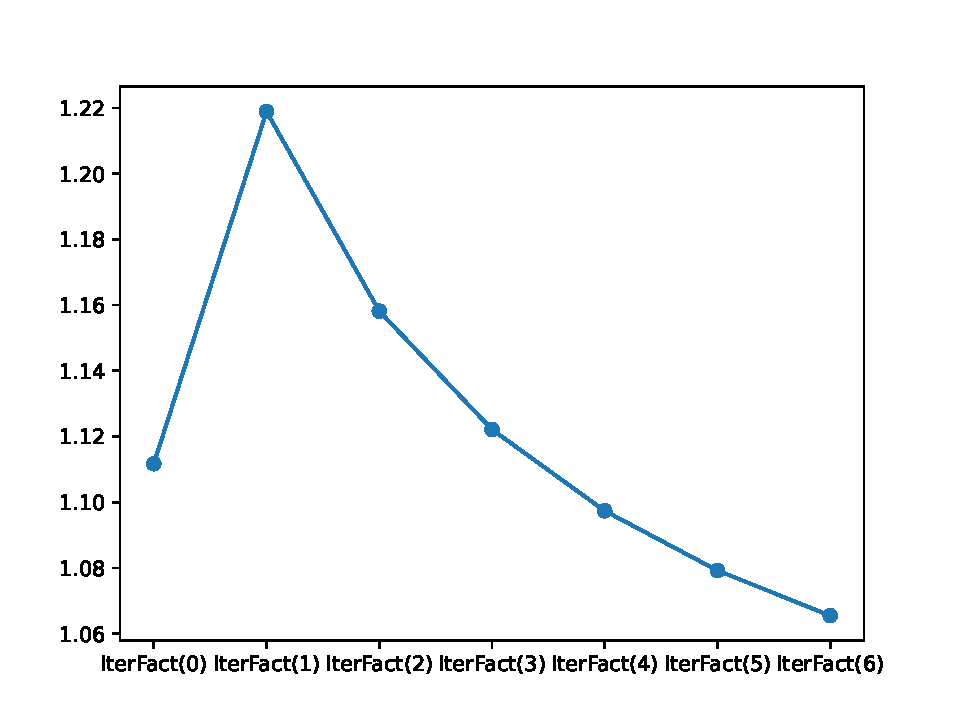
\includegraphics[width=0.8\linewidth, page=1]{Figures.pdf}
    \end{center}
    \caption{Отношение количества малых шагов при использовании параллельного набора правил вычисления аргументов и последовательного}
    \label{fig:fact_total}
\end{figure}

Так, на рисунке~\ref{fig:fact_total} изображен график отношения количества малых шагов при использовании параллельного набора правил вычисления аргументов и последовательного.
По нему можно сделать вывод о том, что использование параллельного набора правил при небольшом объеме вычислений привносит дополнительные редукции, но с усложнением программы количество дополнительных редукций становится мало в процентном соотношении.

\begin{figure}
    \begin{center}
        \includegraphics[width=0.8\linewidth, page=2]{Figures.pdf}
    \end{center}
    \caption{Отношение количества больших шагов при использовании последовательного набора правил вычисления аргументов и параллельного}
    \label{fig:fact_height}
\end{figure}

На рисунке~\ref{fig:fact_height} же представлен график отношения количества больших шагов при использовании последовательного набора правил вычисления аргументов и параллельного.
На его основе можно сделать вывод, что параллельный набор правил даёт значительное ускорение (порядка 1.67 раз) при наличии нужного количества исполнителей малого шага.

\begin{figure}
    \begin{center}
        \includegraphics[width=0.8\linewidth, page=3]{Figures.pdf}
    \end{center}
    \caption{Распределение ширин большого шага}
    \label{fig:fact_distr}
\end{figure}

Рисунок~\ref{fig:fact_distr} построен следующим образом: для каждого большого шага была измерена его ширина, затем посчитано сколько раз каждая ширина встречалась среди всех шагов, и затем построена гистограмма.
Несмотря на то, что во всех случаях чаще всего ширина большого шага~--- 1, в параллельном наборе правил ширина от 2 до 20 наблюдается гораздо чаще, чем при использовании последовательного, что позволяет говорить о том, что параллельный набор правил увеличивает параллельность.

\begin{figure}
    \begin{center}
        \includegraphics[width=0.8\linewidth, page=4]{Figures.pdf}
    \end{center}
    \caption{График количества больших и малых шагов}
    \label{fig:fact_red}
\end{figure}

На рисунке~\ref{fig:fact_red} изображен сводный график количества больших и малых шагов.

\paragraph{Выводы.}

Тестирование позволило оценить текущее состояние проекта: программный стек целиком работоспособен, хоть и требует доработки.
Б\'ольшая часть проблем оказалась связана с ограничениями существующих схем трансляции $\lambda$-термов в \INs{}, в частности, с отсутствием поддержки числовых литералов и алгебраических типов данных.
Тем не менее, полученная статистика исполнения позволяет говорить о том, что трансляция $\lambda$-термов в \INs{} позволяет достаточно эффективно редуцировать $\lambda$-термы параллельно, при использовании соответствующих схем трансляции и наборов правил.
